\documentclass{article}
\usepackage{amsmath}
\usepackage{amsfonts}
\usepackage{amssymb}
\usepackage{enumitem}
\usepackage{tikz}
\usepackage{mathtools}

\usetikzlibrary{arrows}

\title{MATH 222 - Assignment 4}
\date{March 2017}
\author{Daniel Frankcom}

\begin{document}
	\pagenumbering{gobble}
	\maketitle
	\setlength{\parindent}{0pt}
	\newcommand{\forceindent}{\leavevmode{\parindent=72pt\indent}}
	\newpage
	\pagenumbering{arabic}
	
	\begin{enumerate}
		
		\item 
		\begin{enumerate}
			\item In order for a relation to be both symmetric and antisymmetric, it must only contain reflexive elements. For each reflexive pair $(x,x)$, there are 2 options: either the pair is in the relation, or it is not.
			\newline $\therefore$ there are $2^n$ relations on $A$ that fulfill the requirements
			\item If $R$ is a relation on $A$ that is antisymmetric, then it may not contain any 2 pairs such that $(x,y)$ and $(y,x)$ are both in $R$ unless $x=y$.
			\newline $\therefore$ we can count the number of elements in the upper diagonal half of the corresponding relation matrix.
			\newline This is equivalent to $\sum\limits_{i=1}^{n}i=\frac{n(n+1)}{2}$
			\item For each pair, either $(x,y)$ or $(y,x)$ may be in $R$, unless $x=y$.
			\newline $\therefore$ there are $\frac{n(n+1)}{2}-n=\frac{n(n-1)}{2}$ pairs that may be swapped out for their inverse.
			\newline As in part (a), we have 2 options for each of our pairs, so we have $2^\frac{n(n-1)}{2}$ relations
			\item If $R$ has domain $A$ and is a function, then each element may map to only 1 other element in $A$, by the definition of a function. 
			\newline Since $R$ is reflexive, for every $x\in A$ the pair $(x,x)$ must be in $R$.
			\newline Since every value in the domain is already mapped to itself, we know that no value can map to another due to our function restriction.
			\newline $\therefore R$ is made up of all of the reflexive pairs $(x,x)$ where $x\in A$
		\end{enumerate}
	
		\item 
		\begin{enumerate}
			\item \mbox{}
			\newline
			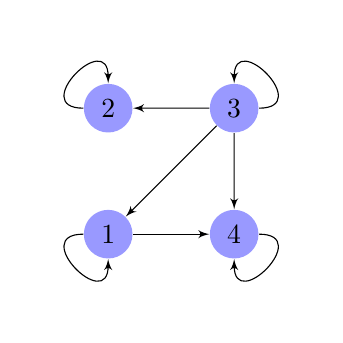
\begin{tikzpicture}
			[scale=.8,auto=left,every node/.style={circle,fill=blue!40}, edge/.style={->,> = latex'}]
			\node (n1) at (0,0)  {1};
			\node (n2) at (0,2)  {2};
			\node (n3) at (2,2)  {3};
			\node (n4) at (2,0)  {4};
			
			\foreach \from/\to in {n1/n4,n3/n4,n3/n1,n3/n2}
			\draw[edge] (\from) to (\to);
			
			\draw[edge] (n1) to [out=180,in=270,looseness=4] (n1);
			\draw[edge] (n2) to [out=180,in=90,looseness=4] (n2);
			\draw[edge] (n3) to [out=360,in=90,looseness=4] (n3);
			\draw[edge] (n4) to [out=360,in=270,looseness=4] (n4);
			\end{tikzpicture}
			
			\item \mbox{}
			\newline
			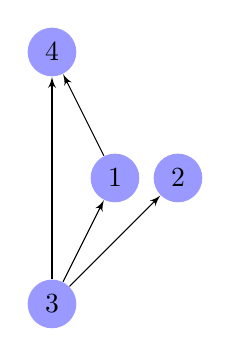
\begin{tikzpicture}
			[scale=.8,auto=left,every node/.style={circle,fill=blue!40}, edge/.style={->,> = latex'}]
			\node (n1) at (1,2)  {1};
			\node (n2) at (2,2)  {2};
			\node (n3) at (0,0)  {3};
			\node (n4) at (0,4)  {4};
			
			\foreach \from/\to in {n1/n4,n3/n4,n3/n1,n3/n2}
			\draw[edge] (\from) to (\to);

			\end{tikzpicture}
		\end{enumerate}
	
	\end{enumerate}
\end{document}